% ---
% Arquivo com a revisão bibliográfica do Trabalho de Conclusão de Curso dos alunos
% Gabriel Takaoka Nishimura, Felippe Demarqui Ramos e Vivian Kimie Isuyama 
% da Escola Politécnica da Universidade de São Paulo
% ---
	\chapter{Revisão Bibliográfica}\label{cap-revisao-bibliografica}
	
	Nesse capítulo será feita a verificação do estado atual de outros trabalhos sobre comunicação via luz. Serão analisados tanto o meio comercial quanto o acadêmico.
	
	\section{Lifi-X}
	
	A única solução de VLC anunciada disponível no mercado é o LiFi-X, de uma empresa chamada \textit{pureLifi}. Que afirma fornecer:
	
	\begin{itemize}
		\item Comunicação \textit{full duplex} com 40Mpbs de \textit{download} e \textit{upload};
		\item Módulo receptor portátil ligado via USB;
		\item Múltiplos usuários por ponto de acesso;
		\item \textit{Handover} suportado entre múltiplos pontos de acesso;
		\item Comunicação sem fio segura contida por paredes;
	\end{itemize}

	A descrição do produto não especifica a modulação utilizada, ou se existe algum código de correção de erro implementado. Sua velocidade de \textit{download} é comparável ao 802.15.11g, que tem velocidades teóricas de 54Mpbs. Entretanto, o produto está em fase de lançamento então não tem preço de venda ainda.

	\section{Franhoufer-Gesellschaft}\label{section:fraunhofer}
	
	Antes da publicação da norma IEEE 802.15.7 em Setembro de 2011, o Fraunhofer-Gesellschaft conseguiu criar um link de 513 Mbit/s utilizando VLC \cite{513mb-fraunhofer}. A implementação utilizou modulação baseada em DMT (Discrete Multi-Tone) e QAM (Quadrature Amplitude Modulation), assim como técnicas de \textit{bit} e \textit{power loading} e \textit{clipping} simétrico.
		
	É utilizado um LED de alta potência para iluminar o receptor com 1000 lx e transmitir os dados modulados. Para possibilitar isso, o circuito analógico de transmissão utiliza um Bias-T, que adiciona uma componente de corrente contínua (DC) a uma onda com a mensagem codificada. A componente DC mantém a iluminação alta enquanto a mensagem é enviada ao receptor, que recebe os sinais luminosos com um fotodiodo e remove a componente de iluminação utilizando um filtro passa-baixas, facilitando o processo de recepção e decodificação. A \autoref{figure:fraunhofer-architecture} ilustra a arquitetura do sistema desenvolvido.
	
	\begin{figure}[h]
		\caption{\label{figure:fraunhofer-architecture}Arquitetura do sistema VLC do Instituto Fraunhofer}
		\centering
		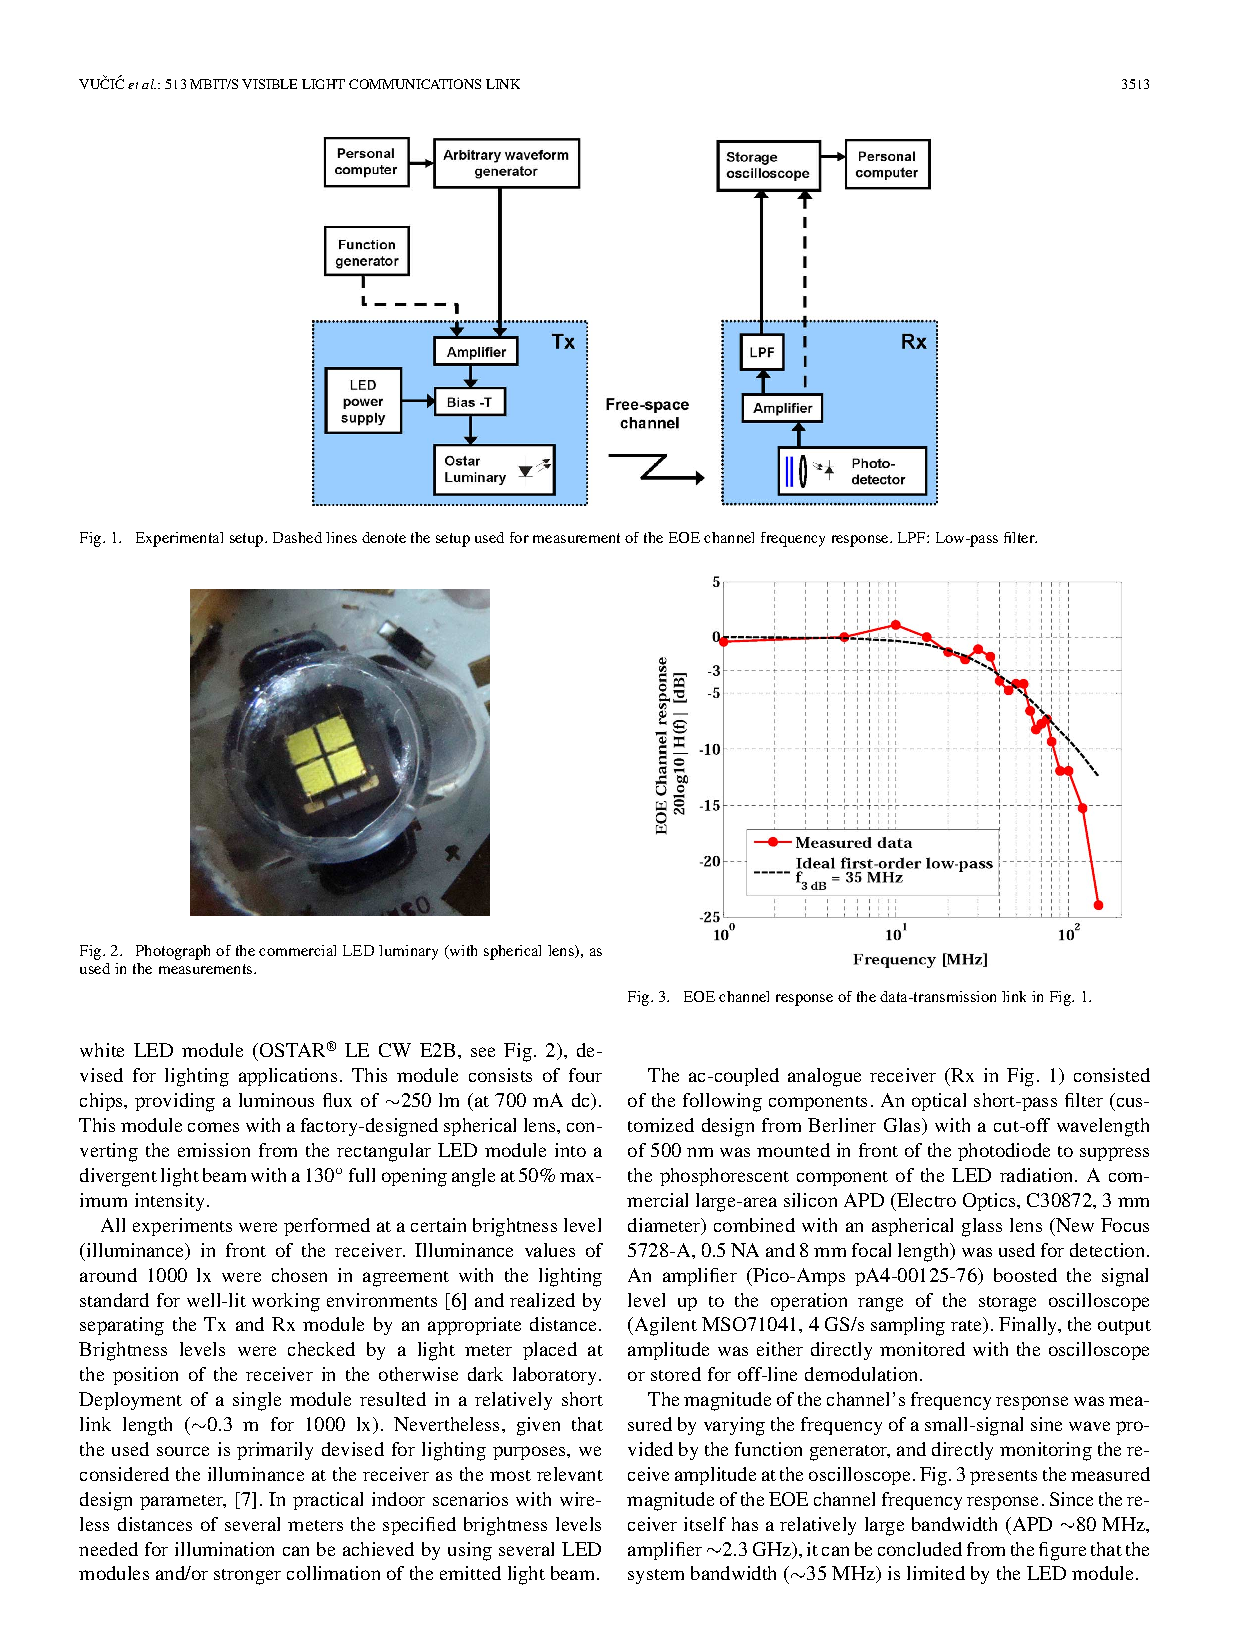
\includegraphics[width=0.8\textwidth, trim={5cm 19.3cm 4.5cm 2cm},clip]{fraunhofer2.pdf}
		\legend{\cite{513mb-fraunhofer}}
	\end{figure}
	
	O \textit{overhead} de transmissão e recepção é removido com o pré e pós-processamento de dados: para transmitir é utilizado um gerador de funções programado com o \textit{payload} e para receber é utilizado um osciloscópio com memória conectado a um computador, onde é realizada uma análise \textit{offline} dos dados.	
	
	O artigo foca no estudo da eficácia das modulações citadas, de forma a obter uma relação distância de transmissão e vazão de dados boa. Ao fim do estudo, foram obtidas vazões de 513 Mbit/s a 30 centímetros de distância. 

	\section{Scuola Superiore Sant’Anna}
	
	Em 2012, a Scuola Superiore Sant’Anna na Itália provou possível a transmissão de 3.4 Gbit/s com distâncias abaixo de 30cm \cite{3.4g-sant-ana}. O artigo se focou na transmissão de luz com modulação WDM (Wavelength Division Multiplexing) utilizando um LED Vermelho Verde e Azul (RGB). Cada comprimento de onda foi então modulado utilizando DMT, que divide o sinal em 512 portadoras, combinadas utilizando QAM.
	
	\begin{figure}[h]
		\caption{\label{figure:santanna-architecture}Configuração experimental da transmissão WDM. AWG: Gerador de Funções; APD: Fotodiodo de Avalanche}
		\centering
		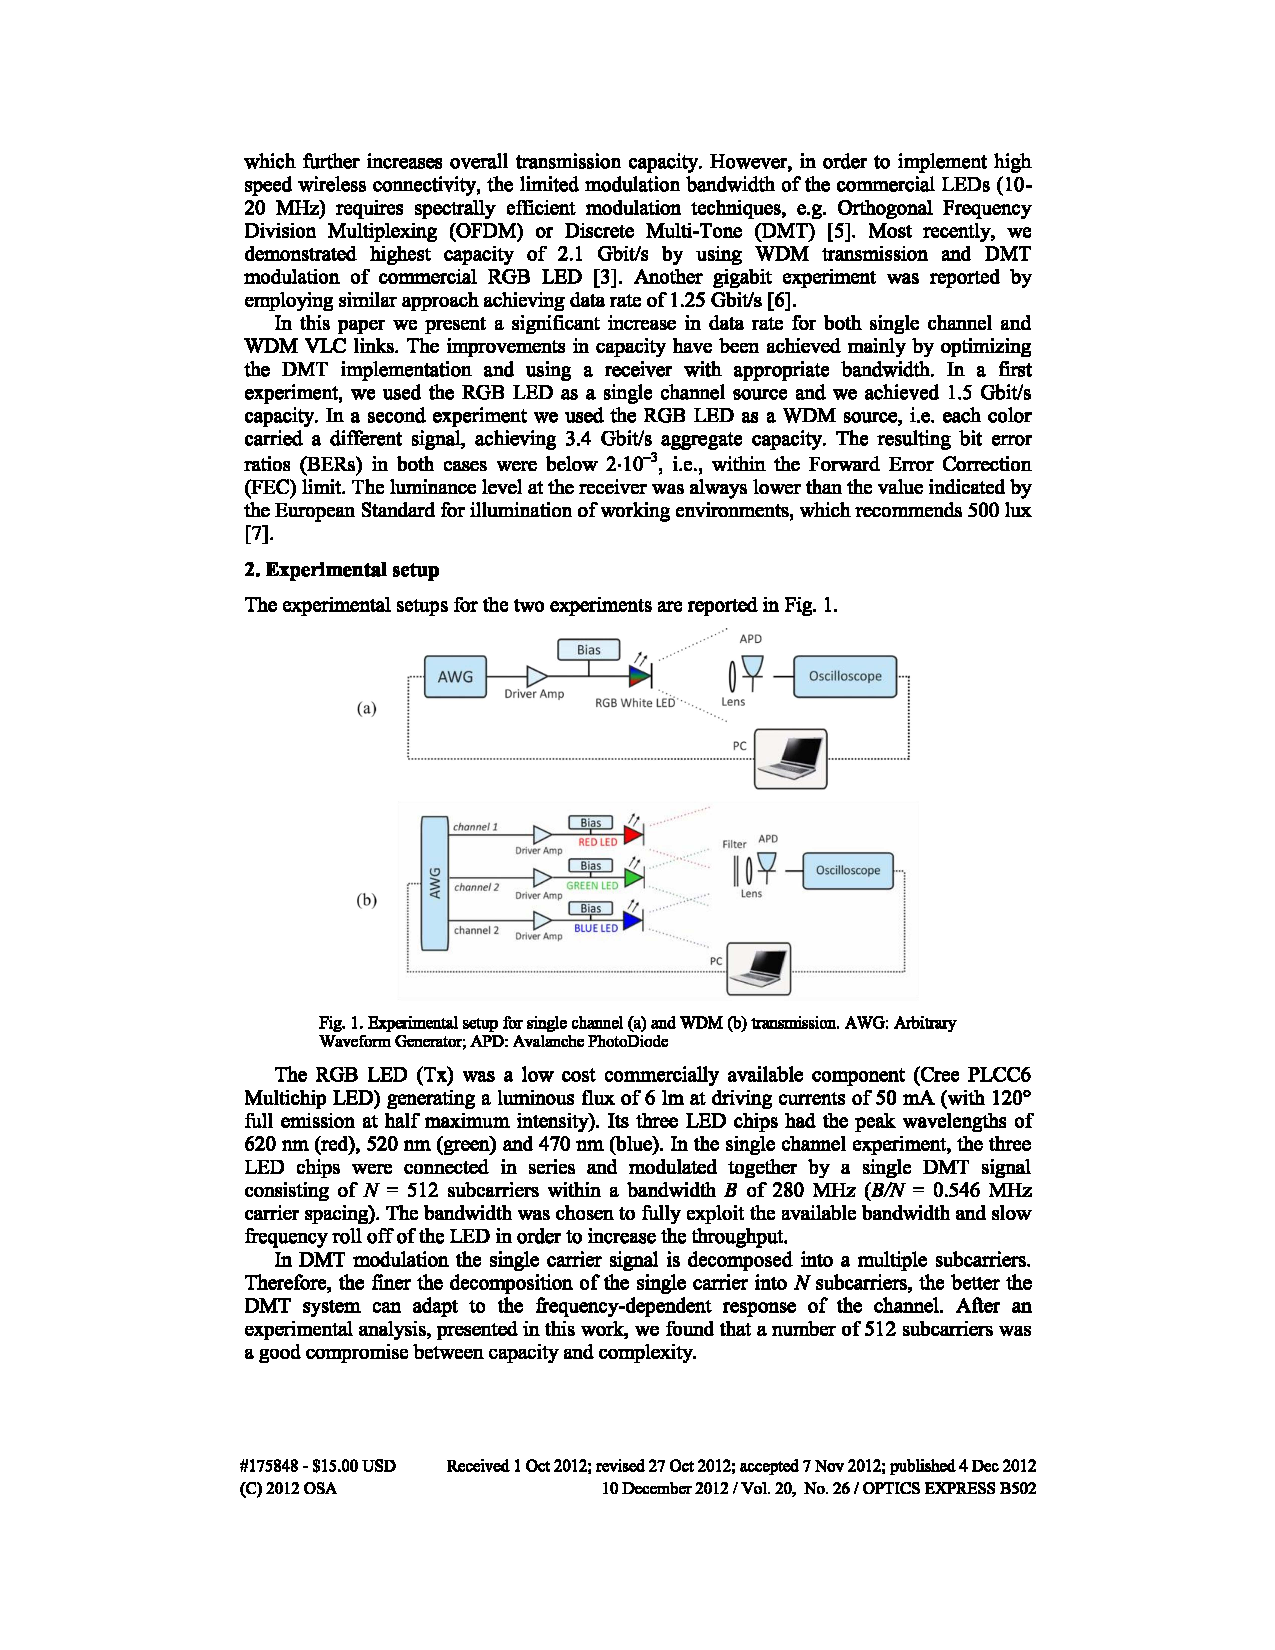
\includegraphics[width=0.8\textwidth, trim={6.6cm 11cm 5cm 13.5cm},clip]{sant-ana.pdf}
		\legend{\cite{3.4g-sant-ana}}
	\end{figure}
	
	Como no artigo anterior (\autoref{section:fraunhofer}), os autores da Scuona Superiore Sant’Ana apenas consideraram a camada física, previamente gravando a mensagem em um gerador de funções para diminição do \textit{overhead}. 
	
	As distâncias obtidas foram de 30cm, com níveis de iluminação de 410 lx no receptor. Como os níveis estavam abaixo do recomendado pela norma Européia para iluminação - que é 500 lx -, foi sugerido que em trabalhos futuros fossem adicionados mais componentes LED do lado do transmissor.
	
	\section{Fudan University}
	
	Três anos depois, na China, a Universidade de Fudan publicou um artigo sobre comunicação via luz a uma taxa de 4.5 Gbit/s \cite{4.5g-fudan}. O artigo se focou em resolver o problema da baixa distância de transmissão em sistemas VLC com velocidades na ordem de grandeza de \textit{Gigabits}/s. Os LEDs utilizados estão disponíveis comercialmente.
	
	Em sistemas de VLC de alta velocidade, a interferência inter-símbolo (ISI) é induzida pela dispersão multi-caminho ótica, degradando a performance do sistema e reduzindo a distância de transmissão. Para reduzir o ISI, os autores propõe a utilização de um equalizador adaptativo baseado no algoritmo \textit{Recursive Least Square} (RLS), devido à suas vantagens sobre outro algoritmo equalizador chamado \textit{Modified Cascaded Multi-Modulus Algorithm} (M-CMMA). Algumas das vantagens do RLS sobre o M-CMMA são a velocidade de convergência do algoritmo e a complexidade computacional total.
	
	Além da etapa de equalização dos sistemas, ainda é descrita a modulação aplicada à mensagem. A sequência de bits da mensagem é mapeado para símbolos complexos em 64QAM, que são posteriormente enviados para modulação \textit{Carrier-less amplitude and phase} (CAP). No artigo, são explicados ainda os motivos da escolha da modulação CAP sobre a \textit{Orthgonal Frequency Divided Multiplexing} OFDM. Utilizando CAP, não é necessária a conversão elétrica ou ótica de números complexos para reais, além de dispensar a transformação de Fourier discreta, reduzindo a complexidade da computação e estrutura do sistema consideravelmente. A arquitetura do sistema e algumas fotos podem ser observadas na \autoref{figure:fudan-architecture}.
	
	\begin{figure}[h]
		\caption{\label{figure:fudan-architecture}Arquitetura do sistema VLC desenvolvido pela Universidade de Fudan. Observa-se a modulação por comprimento de onda com as três cores do LED e o processamento adicional para converter os símbolos em CAP.}
		\centering
		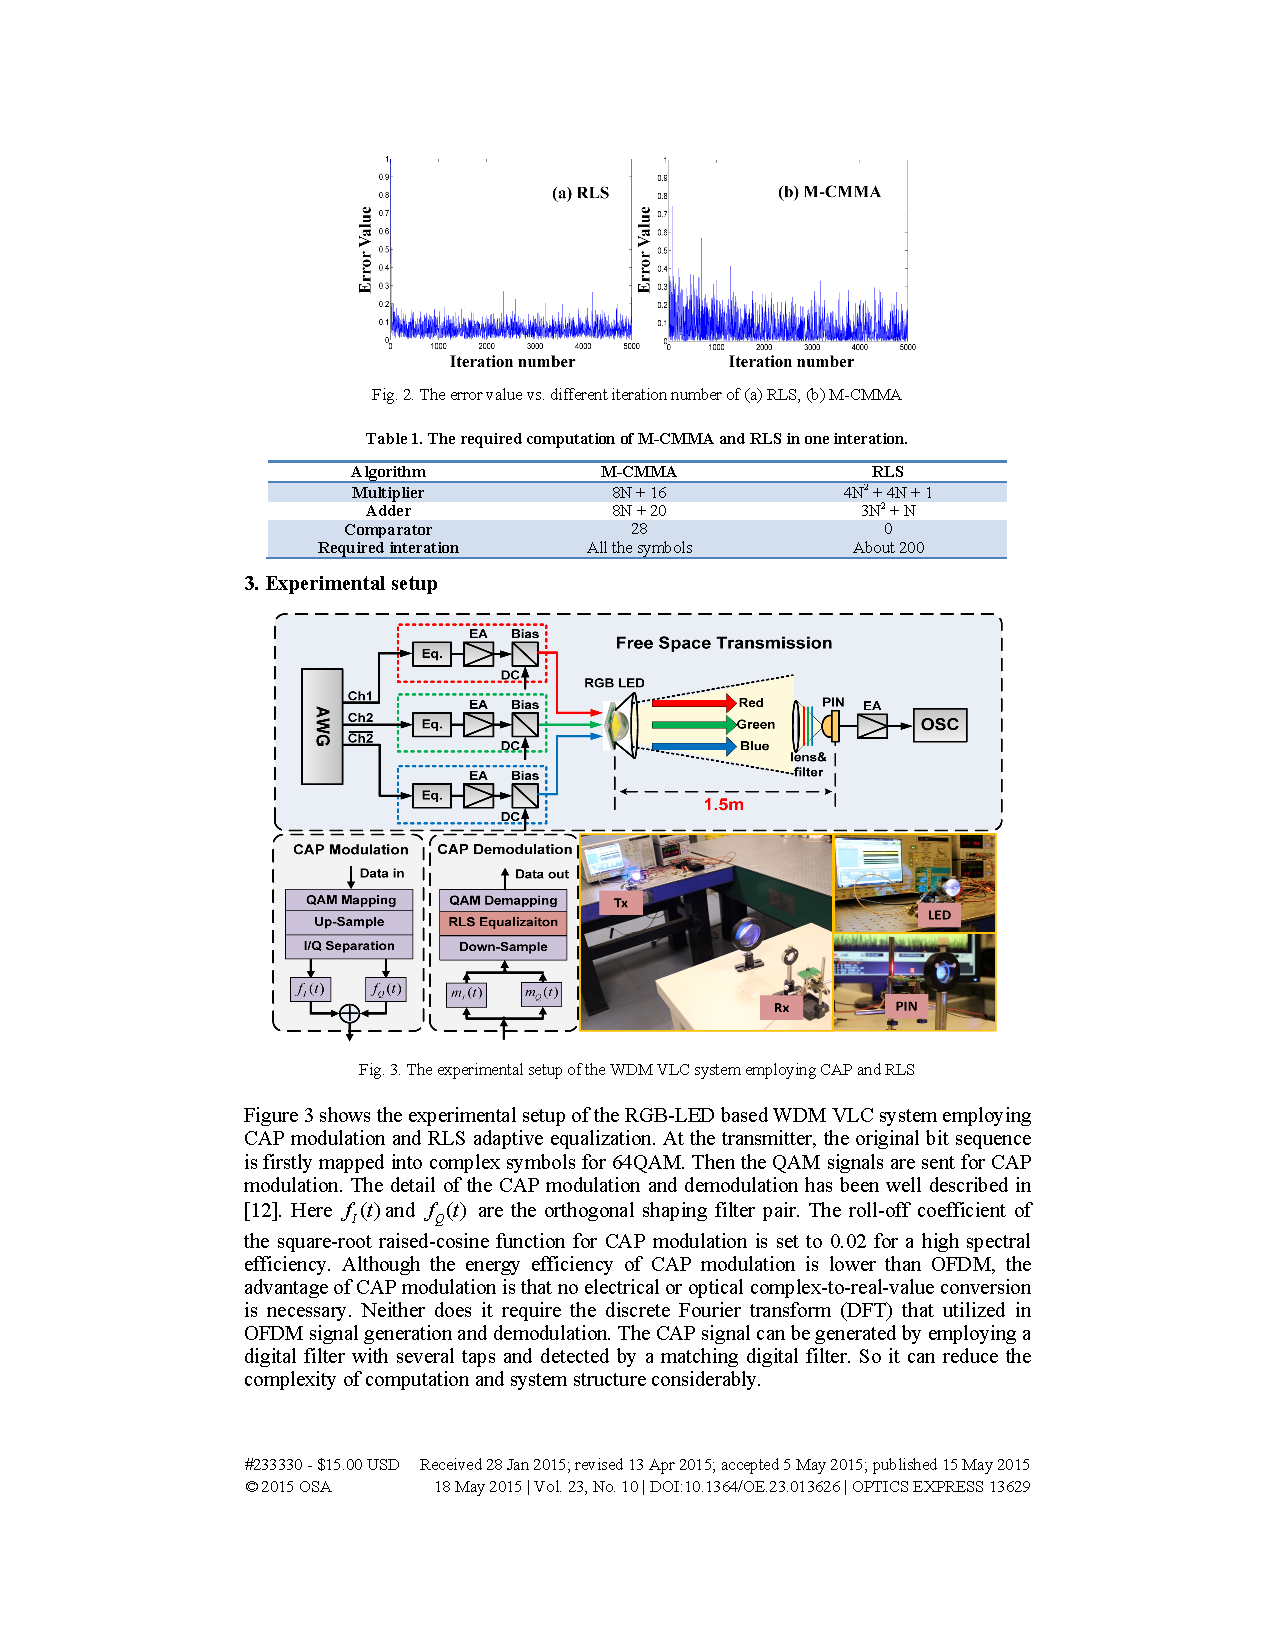
\includegraphics[width=0.8\textwidth, trim={5cm 10cm 5cm 10.1cm},clip]{fudan4.pdf}
		\legend{\cite{4.5g-fudan}}
	\end{figure}
	
	Após as etapas de equalização e modulação, o sistema obteve até 1.5m de distância entre o transmissor e receptor, com taxas de BER 7\% abaixo de 3.8x10e-3.